\HdrGrowthArrayImpl

The following diagrams should provide intuition on how growth arrays work.

\begin{figure}[H]
\label{fig:1}
	\centering{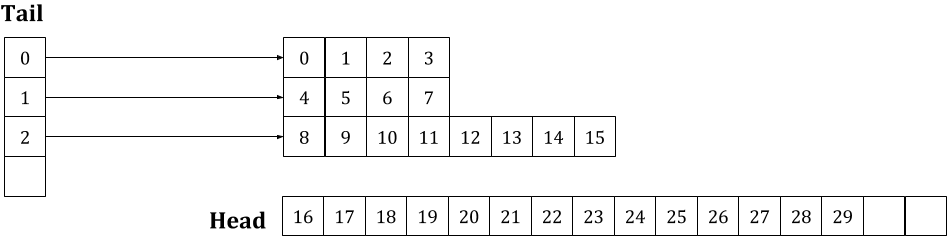
\includegraphics[width=5in]{GrowthArrayDiagram}}
	\caption{Appending $30$ items to a growth array with $\VarInitCapacity = 4$, $\VarGrowthFactor = 2$}
\end{figure}

\begin{figure}[H]
\label{fig:2}
	\centering{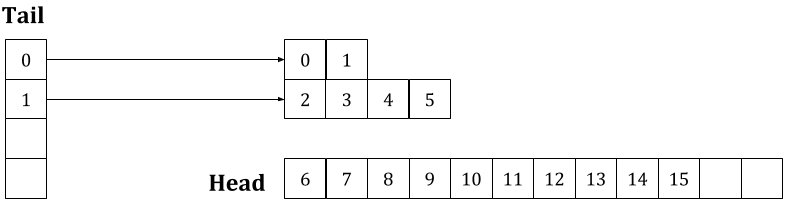
\includegraphics[width=5in]{GrowthArrayDiagram2}}
	\caption{Appending $16$ items to a growth array with $\VarInitCapacity = 2$, $\VarGrowthFactor = 3$}
\end{figure}

\begin{figure}[H]
\label{fig:3}
	\centering{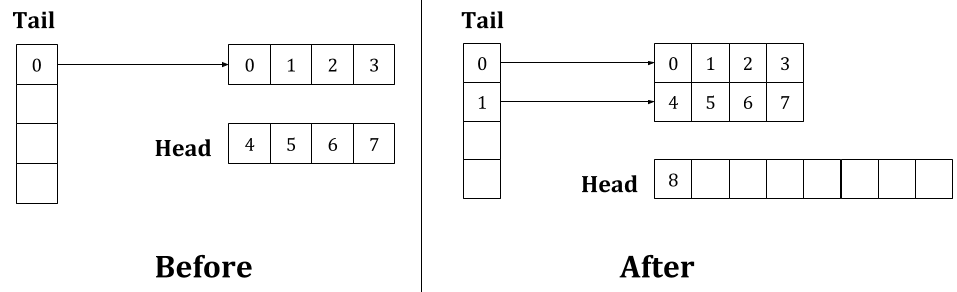
\includegraphics[width=5in]{GrowthArrayDiagram3}}
	\caption{Appending $1$ item to a growth array with $\VarInitCapacity = 4, \VarGrowthFactor = 2$. Initial size: $8$}
\end{figure}

In this section, $\VarList$ denotes a growth array. The following algorithm implements appending for growth arrays.

\begin{algorithm}[H]
	\caption{Appending \TextGrowthArray}
	\begin{algorithmic}[1]
		\Procedure{$\FuncAppend$}{$\VarList,\ \ParamItem$}
			\If{$\VarList.\FieldFull$}
				\State $\VarList.\FuncGrow()$
			\EndIf
		
			\State $\VarList.\FieldHead[\VarList.\FieldHeadSize] \gets \ParamItem$
			\State $\VarList.\FieldSize \gets \VarList.\FieldSize + 1$
		\EndProcedure
		\Statex
		\Procedure{$\FuncGrow$}{$\VarList$}
			\State $\VarList.\FieldTail.Append(\VarList.\FieldHead)$
			\If{$\VarList.\FieldCapacity = \VarInitCapacity$}
				\State $\LclNewHeadCapacity \gets (\VarGrowthFactor - 1) \times \VarInitCapacity$
			\Else
				\State $\LclNewHeadCapacity \gets \VarGrowthFactor \times \VarList.\FieldHeadCapacity$
			\EndIf
			\State $\VarList.\FieldHead \gets \FuncNewArray(\LclNewHeadCapacity)$
			\State $\VarList.\FieldCapacity \gets \VarList.\FieldCapacity + \LclNewHeadCapacity$
		\EndProcedure
	\end{algorithmic}
\end{algorithm}

\HdrTimeComplex

It takes $O(n)$ time to append $n$ items to a growth array. This can be easily seen by noting that every statement in the algorithm has amortized $O(1)$ time complexity (ignoring the call to $\FuncNewArray$, since memory allocation is non-deterministic).

Now, I focus on finding a formula for growth arrays' write cost function, $\FuncWritesGrowthArray(n)$, which will be written as $\FuncWrites(n)$ in this section. I claim that Lemma \ref{lem:CapacitySeq} also holds for growth arrays, since they satisfy all properties used by that proof. In particular, although growth arrays use a different growth algorithm than dynamic arrays, they still have the following property:

\begin{lemma}
\label{lem:GrowthArraysGrowthFactor}
	The capacity of a growth array grows by the constant factor $\VarGrowthFactor$.
\end{lemma}

\begin{proof}
	I prove that the $\FuncGrow$ algorithm enforces this using induction. I induct on the number of times $\FuncGrow$ is called, $k$, showing that for all natural numbers $k$, $\FuncGrow$ behaves correctly when called the $k$th time. I will let $c_i$ and $c_f$ denote the initial/final capacities and $h_i$ and $h_f$ denote the initial/final head capacities for the $k$th call, respectively.

	For $k = 1$, $c_i = \VarInitCapacity$. I wish to show that $c_f = \VarGrowthFactor\VarInitCapacity$. This happens if and only if the next buffer has size $\Delta c = (\VarGrowthFactor - 1)\VarInitCapacity$, which the algorithm ensures.
	
	For $k > 1$, by induction $c_i = \text{previous }c_f = \VarGrowthFactor^{k - 1}\VarInitCapacity$, and $h_i = \text{previous }h_f = (\VarGrowthFactor^{k - 1} - \VarGrowthFactor^{k - 2})\VarInitCapacity$. I wish to show $c_f = \VarGrowthFactor^{k}\VarInitCapacity$ and $h_f = (\VarGrowthFactor^{k} - \VarGrowthFactor^{k - 1})\VarInitCapacity$. Because $k > 1$, the algorithm will calculate $h_f$ as $\VarGrowthFactor$ times $h_i$. Then
	\begin{align*}
	h_f &= \VarGrowthFactor h_i = \VarGrowthFactor (\VarGrowthFactor^{k - 1} - \VarGrowthFactor^{k - 2})\VarInitCapacity = (\VarGrowthFactor^{k} - \VarGrowthFactor^{k - 1})\VarInitCapacity
	\end{align*}
	and
	\begin{align*}
	c_f &= c_i + h_f = \VarGrowthFactor^{k - 1}\VarInitCapacity + (\VarGrowthFactor^{k} - \VarGrowthFactor^{k - 1})\VarInitCapacity = \VarGrowthFactor^{k}\VarInitCapacity
	\end{align*}
	as desired.
\end{proof}

Since Lemma \ref{lem:GrowthArraysGrowthFactor} has been proven, Lemma \ref{lem:CapacitySeq} and all results based on it must also hold true for growth arrays. Now, I am ready to find the write cost of $\FuncGrow$. Unlike dynamic arrays, $\FuncGrow$ does not make $\VarGrowSeq_i$ writes when the current size is $\VarGrowSeq_i$. In fact, $\FuncGrow$ does not copy \textit{any} items supplied by the user. Writes are only made when a buffer pointer is appended to the tail, since the tail is a dynamic array.

Let $\FuncWritesByGrow(n)$ denote the total number of writes made by $\FuncGrow$, and let $\VarNumPointersTail$ be the size of the tail. Since Corollary \ref{coro:GrowthSeq} also holds for growth arrays, $\FuncGrow$ is called $|\VarGrowSeq|$ times. A buffer is appended to the tail each time $\FuncGrow$ is called. Thus, the tail's size is
\begin{align*}
\VarNumPointersTail &= |\VarGrowSeq| = |\VarCapacitySeq| - 1 = \VarUseful
\end{align*}
Then the formula for $\FuncWritesByGrow(n)$ is simply $\FuncWritesTail(\VarUseful)$, since $\VarUseful$ pointers are appended to the tail, which is a dynamic array. Finally, adding the writes made by $\FuncAppend$, the formula for $\FuncWrites(n)$ is
\begin{align*}
\FuncWrites(n) = n + \FuncWritesTail(\VarUseful)
\end{align*}
Now, I approximate $\FuncWrites(n)$ using $\sim$. To do this, I will derive the big-O complexity of $\VarUseful$.

\begin{lemma}
\label{lem:VarUsefulIsOLogN}
	$\VarUseful = O(\log n)$.
\end{lemma}

\begin{proof}
	From Lemma \ref{lem:CapacitySeq}, $\VarUseful = \max(\ExprMessy, 0)$. For sufficiently large $n$, $\VarUseful = \ExprMessy$. Using $\sim$ to analyze $\VarUseful$, I receive
	\begin{align*}
	\VarUseful \sim \ExprMessy \sim \left( \ExprMessyInner \right) \sim \log_{\VarGrowthFactor} n
	\end{align*}
	(It is trivial to show that $\left\lceil f(n) \right\rceil \sim f(n)$ if $f$ is unbounded, since $\left\lceil f(n) \right\rceil - f(n)$ is bounded by $1$.)
	
	By Theorem \ref{thm:SameBigOClass}, $O(\VarUseful) = O(\log_{\VarGrowthFactor} n) = O(\log n)$ as desired.
\end{proof}

Now when $\FuncWrites(n)$ is approximated with $\sim$, $\FuncWritesTail(\VarUseful)$ disappears:
\begin{align*}
\FuncWrites(n) &= n + \FuncWritesTail(\VarUseful) = n + O(\VarUseful) = n + O(\log n) \sim n
\end{align*}
(The last step is justified by Theorem \ref{thm:RemovesLowerOrderTerms}.)

This says that when $n$ items are added, the number of items written is approximately $n$. This is a significant improvement over the asymptotic bounds for $\FuncWritesDynamicArray(n)$.

\HdrSpaceComplex

Unlike dynamic arrays, growth arrays do not throw away buffers. This means that if the current capacity is $c$, then the total length of buffers allocated to store items is also $c$. Typically, however, $\FuncSpace(n) > c$. This is because the tail of growth arrays (which is a dynamic array) also allocates buffers to store buffer pointers. The space the tail allocates must be considered in the formula for $\FuncSpace(n)$.

In the previous section, I established that $\VarNumPointersTail = \VarUseful$. Since $\VarCapacitySeq_\VarUseful$ is the capacity needed to hold $n$ items, and $\FuncSpaceTail(\VarUseful)$ is the space the tail needs to store $\VarUseful$ pointers, I conclude that the formula for $\FuncSpace(n)$ is
\begin{align*}
\FuncSpace(n) = \VarCapacitySeq_\VarUseful + \FuncSpaceTail(\VarUseful)
\end{align*}
($\FuncSpaceTail$ denotes the space cost function for dynamic arrays.)

Now, I wish to approximate this using $\sim$. Since $\VarCapacitySeq_\VarUseful = \VarGrowthFactor^\VarUseful\VarInitCapacity$, it follows from Lemma \ref{lem:ToVarUsefulPowerBounds} that $n \FluteLeq \VarCapacitySeq_\VarUseful \FluteLess \VarGrowthFactor{n}$. From Corollary \ref{coro:BothSidesInequalityInvert}, $\frac{1}{\VarGrowthFactor n} \FluteLess \frac{1}{\VarCapacitySeq_\VarUseful} \FluteLeq \frac{1}{n}$. From Theorem \ref{thm:BothSidesInequality}, $\frac{\FuncSpaceTail(\VarUseful)}{\VarGrowthFactor n} \FluteLess \frac{\FuncSpaceTail(\VarUseful)}{\VarCapacitySeq_\VarUseful} \FluteLeq \frac{\FuncSpaceTail(\VarUseful)}{n}$.

Since $\FuncSpaceTail(\VarUseful) = O(\VarUseful) = O(\log n)$, the limits of the lower and upper bounds are both $0$. From the squeeze theorem, it follows that $\ExprNToInfty \frac{\FuncSpaceTail(\VarUseful)}{\VarCapacitySeq_\VarUseful} = 0$. Thus, $\FuncSpaceTail(\VarUseful) = o(\VarCapacitySeq_\VarUseful)$. From Theorem \ref{thm:RemovesLowerOrderTerms}, one can conclude
\begin{align*}
\FuncSpace(n) = \VarCapacitySeq_\VarUseful + \FuncSpaceTail(\VarUseful) \sim \VarCapacitySeq_\VarUseful
\end{align*}
Using Theorem \ref{thm:InterchangeableInInequality}, I may substitute $\FuncSpace(n)$ for $\VarCapacitySeq_\VarUseful$ in the first inequality to receive
\begin{align*}
n \FluteLeq \FuncSpace(n) \FluteLess \VarGrowthFactor{n}
\end{align*}
This result is significant since it has smaller lower and upper bounds than $\FuncSpaceDynamicArray(n)$. Since the same values of $n$ as for $\FuncSpaceDynamicArray(n)$ correspond to when it is close to the bounds for $\FuncSpace(n)$ (namely, when $n$ is approximately $\VarGrowSeq_i$), $\FuncSpace(n)$ is asymptotically less than $\FuncSpaceDynamicArray(n)$ even though their intervals overlap. This will be proven rigorously in the space complexity comparison section.